\chapter{Sonido, osciladores cuánticos y segunda ley}

\lectureoverview{La segunda ley es nuestro destino, pero dos cálculos concretos nos preparan el camino. La velocidad del sonido muestra cómo las derivadas termodinámicas se convierten en movimiento observable. Después, el oscilador armónico pone de manifiesto el fallo de la equipartición clásica para los grados de libertad rígidos y muestra cómo la mecánica cuántica activa los modos uno a uno. Por último, volvemos al aparente conflicto entre la dinámica microscópica reversible y el aumento de la entropía. Mediante el flujo en el espacio de fases, el coarse-graining, el caos y la recurrencia, formularemos la segunda ley como una ley abrumadoramente probable, no como una prohibición mecánica sin excepciones.}

\section{Una promesa sobre la segunda ley}

El problema central es fácil de plantear y difícil de explicar. Las ecuaciones newtonianas son reversibles: si una historia microscópica es posible, también lo es la historia invertida en el tiempo. Sin embargo, la segunda ley afirma que los procesos macroscópicos tienen una dirección preferente, caracterizada por una entropía que normalmente aumenta. Llegaremos a esa tensión, pero no de inmediato. Primero conviene ver cómo la mecánica estadística produce información concreta y luego encontrarnos, en un cálculo elemental, con el enigma histórico que obligó a la física clásica a ceder ante la física cuántica.

El primer ejemplo es numérico y deliberadamente aproximado: estimar la velocidad del sonido en un gas diluido. El segundo es exacto dentro de sus hipótesis: calcular la energía media de un oscilador armónico en un baño térmico. El oscilador nos llevará de la equipartición a los niveles de energía cuantizados, de un modo a infinitos modos y, finalmente, de vuelta a la pregunta de qué significa que un sistema de muchas partículas olvide su estado inicial.

\section{La escala molecular de la velocidad del sonido}

Imaginemos una pequeña sobredensidad en un gas diluido. Se dispersa porque las moléculas abandonan la región congestionada, así que su velocidad de propagación debería ser comparable a la velocidad molecular. La equipartición da la energía cinética de una molécula, \begin{equation}
 \frac{3}{2}k_B T
 =\frac{1}{2}m\expect{v^2},
 \qquad
 \expect{v^2}=\frac{3k_B T}{m}.
 \label{eq:sm7-molecular-speed}
\end{equation}Aquí la temperatura se mide desde el cero absoluto y se ha restituido \(k_B\) porque queremos usar unidades de laboratorio. El argumento solo proporciona una estimación de escala: la velocidad cuadrática media de las moléculas no es, por sí misma, la velocidad de una onda sonora colectiva.

Una derivación más sistemática considera un pequeño elemento de gas. Las presiones desiguales en sus caras opuestas ejercen una fuerza neta, y su aceleración es inversamente proporcional a la densidad de masa. El resultado tiene la forma \begin{equation}
 c_s^2=
 \left(\frac{\partial P}{\partial \rho_m}\right)_{\cal C},
 \qquad
 \rho_m=m\rho,
 \label{eq:sm7-sound-general}
\end{equation}donde \(\rho\) es la densidad numérica y el subíndice \({\cal C}\) especifica la condición termodinámica que sigue la perturbación. El cálculo en la pizarra usa \begin{equation}
 P=\rho k_B T
 \quad\Longrightarrow\quad
 \frac{1}{m}
 \left(\frac{\partial P}{\partial\rho}\right)_T
 =\frac{k_B T}{m}.
 \label{eq:sm7-sound-isothermal}
\end{equation}Esta es la estimación isotérmica de la velocidad del sonido. Difiere de \eqref{eq:sm7-molecular-speed} en un factor de \(3\) para la velocidad al cuadrado, o de \(\sqrt{3}\) para la velocidad.

\begin{figure}[t]\centering
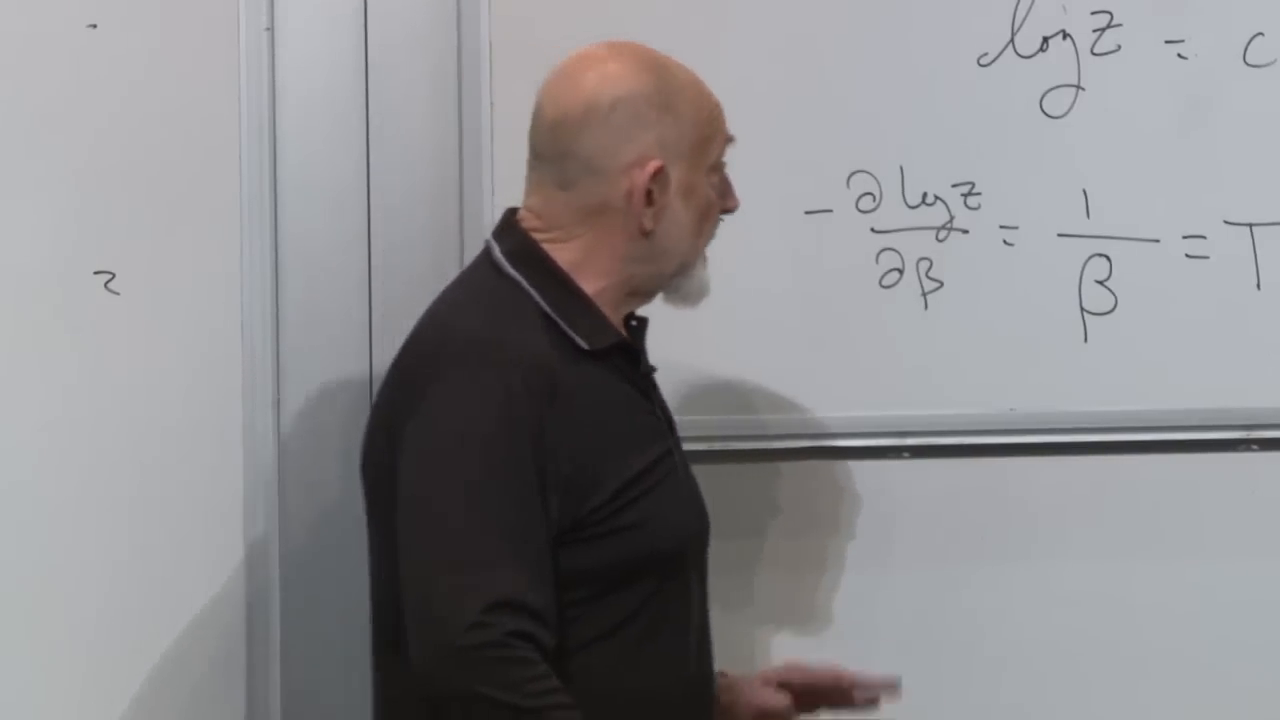
\includegraphics[width=0.90\textwidth]{lecture_07_figure_02.png}\caption{La estimación de la velocidad molecular, la derivada de la presión y la sustitución para un gas ideal, mostradas juntas.}\lectureframe{00:08:55}\end{figure}

Hay una importante precisión que hacer. Una onda sonora de pequeña amplitud suele comprimir y enrarecer el gas más rápido de lo que el calor puede fluir entre elementos vecinos. Por tanto, el movimiento local es aproximadamente adiabático, no isotérmico: \begin{equation}
 c_s^2=
 \left(\frac{\partial P}{\partial\rho_m}\right)_S.
 \label{eq:sm7-sound-adiabatic}
\end{equation}Para un gas ideal con índice adiabático \(\gamma\), \begin{equation}
 P\rho_m^{-\gamma}=\text{constant},
 \qquad
 c_s^2=\gamma\frac{P}{\rho_m}
       =\gamma\frac{k_B T}{m}.
 \label{eq:sm7-sound-ideal-adiabatic}
\end{equation}Para el aire diatómico a temperatura ambiente, \(\gamma\simeq 7/5\). Así, el cálculo a temperatura fija es una primera estimación útil, mientras que la derivada adiabática proporciona la corrección físicamente adecuada.

Con los valores aproximados \begin{equation}
\begin{aligned}
 k_B&\simeq1.3\times10^{-23}\ {\rm J\,K^{-1}},
 &T&\simeq300\ {\rm K},\\
 m_{\rm air}&\simeq4\times10^{-26}\ {\rm kg}.&&
\end{aligned}
 \label{eq:sm7-air-data}
\end{equation}la estimación molecular es de alrededor de \(500\ {\rm m\,s^{-1}}\). Aquí la temperatura debe ser una temperatura absoluta en kelvin, no una escala desplazada como la Fahrenheit. La velocidad del sonido habitual es del orden de \(300\ {\rm m\,s^{-1}}\), y la fórmula adiabática para un gas ideal da aproximadamente \(340\ {\rm m\,s^{-1}}\) a temperatura ambiente. Por tanto, el cálculo aproximado ha encontrado la escala física correcta.

\begin{figure}[t]\centering
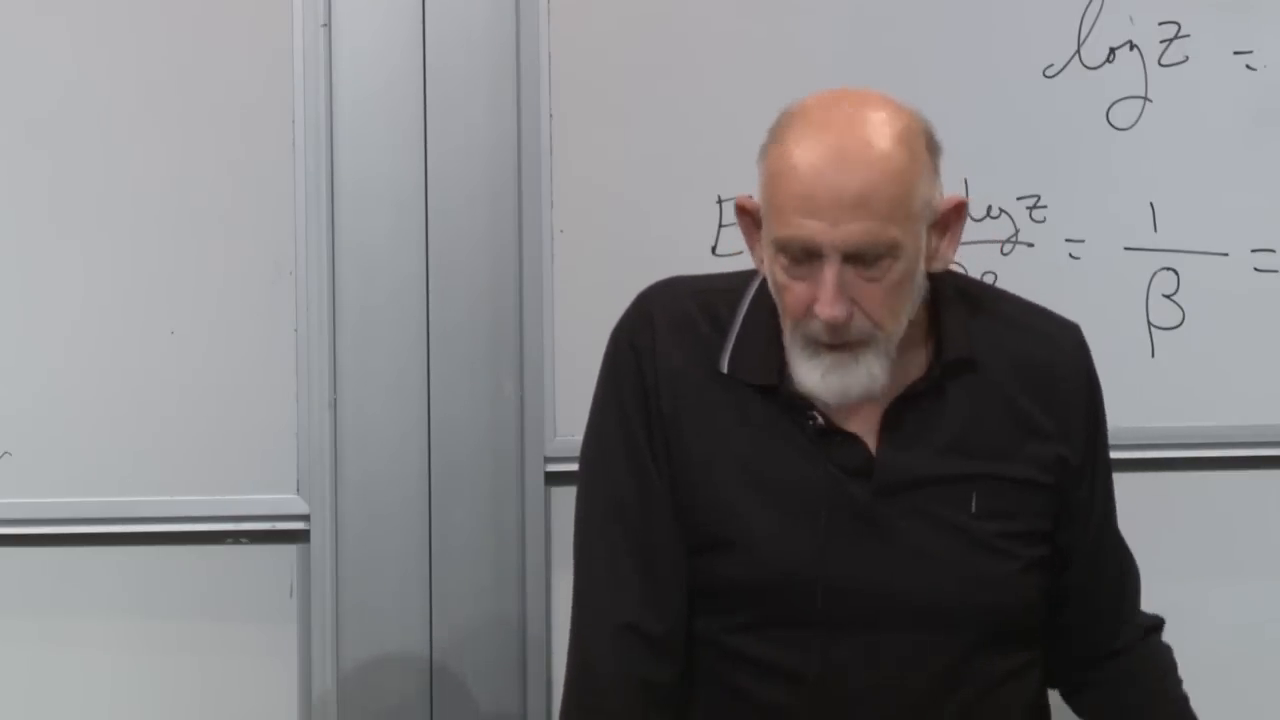
\includegraphics[width=0.90\textwidth]{lecture_07_figure_03.png}\caption{La estimación para el aire a temperatura ambiente usando la constante de Boltzmann, una masa molecular efectiva cercana a \(30\) masas de protón y \(T\simeq300\ {\rm K}\).}\lectureframe{00:10:55}\end{figure}

Mucho antes de que se dispusiera de una descripción microscópica, era posible determinar la velocidad del sonido midiendo la presión en función de la densidad. El argumento estadístico añade la sorprendente interpretación de que la velocidad macroscópica resultante está determinada por la velocidad térmica de las moléculas individuales.

\begin{classroomqa}\audiencequestion{¿Hay que añadir los neutrones a la masa molecular? ¿El número \(14\) del nitrógeno cuenta solo los protones?}\lecturerresponse{El peso atómico citado ya cuenta los protones y los neutrones. El nitrógeno molecular contiene dos átomos de peso atómico cercano a \(14\), así que su masa es de aproximadamente \(28\) masas de protón; para esta estimación basta redondear \(28\) a \(30\).\lecturetimestamp{00:10:58--00:11:16}}\end{classroomqa}

\begin{classroomqa}\audiencequestion{El factor \(3\) proviene de las tres direcciones de traslación, mientras que el sonido se propaga en una sola dirección. ¿Debería esto eliminar el factor \(3\)?}\lecturerresponse{Esto nos advierte correctamente que no debemos identificar la velocidad cuadrática media tridimensional de las moléculas con una velocidad de propagación unidimensional. El argumento inicial solo ofrecía una imagen de orden de magnitud. Una respuesta controlada se obtiene a partir de la derivada de la presión, junto con la condición termodinámica adecuada para la onda.\lecturetimestamp{00:11:12--00:12:00}}\end{classroomqa}

\begin{classroomqa}\audiencequestion{¿La derivada suponía que la temperatura permanece constante durante la onda?}\lecturerresponse{La sustitución para un gas ideal que se muestra sí lo suponía. Mantener fija la temperatura es una estimación provisional plausible para una perturbación muy pequeña; la corrección habitual es que el sonido ordinario es aproximadamente adiabático, lo que sustituye la derivada isotérmica por \(\left(\partial P/\partial\rho_m\right)_S\).\lecturetimestamp{00:12:59--00:14:01}}\end{classroomqa}

\begin{classroomqa}\audiencequestion{Si las variaciones de presión y densidad son ambas pequeñas, ¿su derivada también es pequeña?}\lecturerresponse{No. Una derivada es el cociente de dos variaciones pequeñas en el límite infinitesimal. Tanto \(\delta P\) como \(\delta\rho\) pueden ser pequeñas, mientras que \(\delta P/\delta\rho\) permanece finito y determina la velocidad de la onda.\lecturetimestamp{00:14:03--00:14:23}}\end{classroomqa}

\begin{classroomqa}\audiencequestion{¿Debería aumentar la velocidad del sonido al comprimir el gas, como ocurre al pasar de un gas a un líquido o un sólido?}\lecturerresponse{Sí. La derivada se evalúa en el estado considerado, y \(P(\rho,T)\) no tiene por qué seguir siendo lineal. Cuando las moléculas se comprimen y quedan muy juntas, la ecuación de estado deja de ser ideal y \(\partial P/\partial\rho\) puede crecer considerablemente.\lecturetimestamp{00:14:25--00:15:13}}\end{classroomqa}

\begin{classroomqa}\audiencequestion{¿Puede usarse el valor \(500\ {\rm m\,s^{-1}}\) a cualquier presión?}\lecturerresponse{No. Corresponde al intervalo de baja densidad en el que la ecuación del gas ideal es una aproximación útil. Cuando aparecen potencias superiores de la densidad en \(P(\rho,T)\), la derivada y, por tanto, la velocidad del sonido dependen de la presión y de la densidad.\lecturetimestamp{00:15:14--00:16:29}}\end{classroomqa}

\begin{classroomqa}\audiencequestion{¿También deja de ser válida, al aumentar la densidad, la imagen inicial del sonido propagándose aproximadamente a la velocidad molecular?}\lecturerresponse{Probablemente. Esa imagen está pensada para un gas diluido. Las interacciones colectivas cobran cada vez más importancia a densidad alta, precisamente por lo cual la derivada de la ecuación de estado es una descripción más general.\lecturetimestamp{00:16:32--00:16:53}}\end{classroomqa}

\begin{classroomqa}\audiencequestion{¿Por qué se escribió que la masa de una molécula de nitrógeno es aproximadamente \(30\) masas de protón y no \(28\)?}\lecturerresponse{Solo se necesita la precisión numérica apropiada para la estimación, así que \(28\) se redondeó a \(30\). Dividir también la estimación original de \(500\ {\rm m\,s^{-1}}\) entre \(\sqrt{3}\simeq1.7\) la aproxima a \(300\ {\rm m\,s^{-1}}\), aunque la derivada adiabática es la forma controlada de calcular la corrección.\lecturetimestamp{00:16:54--00:17:27}}\end{classroomqa}

\section{Un oscilador clásico en un baño térmico}

Ahora sustituimos la molécula que se traslada libremente por un oscilador armónico y tratamos todo lo demás como un baño térmico. La imagen inmediata es una masa unida a un resorte, pero el modelo es mucho más amplio. Un modo de una cavidad electromagnética oscila; los átomos de un cristal oscilan; casi cualquier sistema estable desplazado ligeramente del equilibrio ejecuta un movimiento armónico en primera aproximación.

Con \(x\) medido desde el equilibrio, el momento \(p\), la masa \(m\) y la constante del resorte \(\kappa\), el hamiltoniano es \begin{equation}
 H(x,p)=\frac{p^2}{2m}+\frac{\kappa x^2}{2},
 \qquad
 \omega=\sqrt{\frac{\kappa}{m}}.
 \label{eq:sm7-classical-hamiltonian}
\end{equation}El baño fija \(T\) y, a partir de aquí, volvemos a usar \(k_B=1\), de modo que \(\beta=1/T\). Un oscilador en equilibrio con el ambiente tiene una temperatura cercana a \(300\ {\rm K}\); uno sumergido en helio líquido tiene una temperatura de apenas unos kelvin. Un resorte hipotético colocado en el centro del Sol no sobreviviría como resorte, pero el ejemplo aclara el papel del entorno. El factor de Boltzmann se factoriza: \begin{equation}
 e^{-\beta H}
 =e^{-\beta p^2/(2m)}
  e^{-\beta\kappa x^2/2}.
 \label{eq:sm7-factorized-weight}
\end{equation}

\begin{figure}[t]\centering
\includegraphics[width=0.90\textwidth]{lecture_07_figure_04.png}\caption{Un oscilador de masa y resorte, y su hamiltoniano como suma de energía cinética y potencial.}\lectureframe{00:20:55}\end{figure}

A diferencia del gas libre, la integral sobre la posición no da simplemente el volumen del recipiente. El potencial restaurador pondera cada desplazamiento: \begin{equation}
 Z_{\rm cl}
 =\frac{1}{h}\int_{-\infty}^{\infty}dp
             \int_{-\infty}^{\infty}dx\,
 e^{-\beta p^2/(2m)}
 e^{-\beta\kappa x^2/2}.
 \label{eq:sm7-classical-z}
\end{equation}El factor \(1/h\) hace adimensional la función de partición clásica unidimensional. Se omite en el cálculo de la pizarra porque es independiente de \(\beta\) y no puede afectar a la energía media.

\begin{figure}[t]\centering
\includegraphics[width=0.90\textwidth]{lecture_07_figure_05.png}\caption{La función de partición clásica del oscilador, separada en sus integrales gaussianas sobre el momento y el desplazamiento.}\lectureframe{00:22:55}\end{figure}

Para la integral sobre el momento, hacemos el cambio de variable \begin{equation}
 q=\sqrt{\frac{\beta}{2m}}\,p,
 \qquad
 dp=\sqrt{\frac{2m}{\beta}}\,dq.
 \label{eq:sm7-p-gaussian-substitution}
\end{equation}Para la integral sobre la posición, hacemos el cambio de variable \begin{equation}
 y=\sqrt{\frac{\beta\kappa}{2}}\,x,
 \qquad
 dx=\sqrt{\frac{2}{\beta\kappa}}\,dy.
 \label{eq:sm7-x-gaussian-substitution}
\end{equation}Como \(\int_{-\infty}^{\infty}e^{-u^2}\,du=\sqrt{\pi}\), la integral no normalizada sobre el espacio de fases usada en la pizarra es \begin{equation}
 \int dp\,dx\,e^{-\beta H}
 =\frac{2\pi}{\beta}\sqrt{\frac{m}{\kappa}}
 =\frac{2\pi}{\beta\omega}.
 \label{eq:sm7-classical-z-unnormalized}
\end{equation}Al restituir la celda del espacio de fases, \begin{equation}
 Z_{\rm cl}=\frac{2\pi}{h\beta\omega}
           =\frac{1}{\beta\hbar\omega}.
 \label{eq:sm7-classical-z-normalized}
\end{equation}

Para la energía solo importa la dependencia de \(\beta\): \begin{equation}
 \begin{aligned}
 \log Z_{\rm cl}&=\text{constant}-\log\beta,\\
 \expect{H}
 &=-\frac{\partial\log Z_{\rm cl}}{\partial\beta}\\
 &=\frac{1}{\beta}=T.
 \end{aligned}
 \label{eq:sm7-classical-energy}
\end{equation}

\begin{figure}[t]\centering
\includegraphics[width=0.90\textwidth]{lecture_07_figure_06.png}\caption{La cadena clásica completa en la pizarra de la derecha: factorización gaussiana, \(Z\propto(\beta\omega)^{-1}\) y \(\expect{H}=1/\beta=T\).}\lectureframe{00:30:15}\end{figure}

No aparece ningún factor de \(3\) porque se trata de un oscilador espacial. Tampoco queda ningún factor de \(1/2\), porque hay dos términos cuadráticos independientes. Cada gaussiana aporta \(T/2\): \begin{equation}
 \expect{K}=\frac{T}{2},
 \qquad
 \expect{U}=\frac{T}{2},
 \qquad
 \expect{H}=T.
 \label{eq:sm7-equipartition-oscillator}
\end{equation}Esta es la equipartición en su forma más útil: cada término cuadrático independiente del hamiltoniano clásico aporta \(T/2\).

La respuesta es independiente tanto de \(m\) como de \(\kappa\). El movimiento sí depende de esos parámetros: \begin{equation}
 \expect{p^2}=mT,
 \qquad
 \expect{x^2}=\frac{T}{\kappa},
 \qquad
 \expect{\dot{x}^2}=\frac{T}{m}.
 \label{eq:sm7-classical-fluctuations}
\end{equation}Así, una masa mayor se mueve más despacio y un resorte más rígido tiene una amplitud menor, aunque la energía media siga siendo \(T\). Esto resulta inquietante cuando \(\kappa\) se hace descomunalmente grande. Un resorte tan rígido que no pueda moverse debería parecer una restricción congelada; sin embargo, la equipartición clásica todavía le asigna una energía \(T\).

\begin{classroomqa}\audiencequestion{Cuando \(\kappa\to\infty\), la función de partición tiende a cero. ¿Cómo puede seguir usándose su logaritmo?}\lecturerresponse{Mantengamos \(\kappa\) finita, pero arbitrariamente grande. Su contribución a \(\log Z\) es aditiva e independiente de \(\beta\), así que la derivada respecto de \(\beta\) sigue dando \(T\). La inquietud en el límite es real: el cálculo clásico es internamente coherente, pero omite una característica de la naturaleza necesaria para los osciladores muy rígidos.\lecturetimestamp{00:34:01--00:34:54}}\end{classroomqa}

\begin{classroomqa}\audiencequestion{La función de partición del gas ideal requería un \(N!\). ¿Debería aparecer aquí un factorial análogo?}\lecturerresponse{No. Estudiamos un oscilador especificado, no permutamos \(N\) partículas idénticas. Para muchos modos independientes etiquetados, las funciones de partición se multiplican. El factor de indistinguibilidad corresponde a un problema de conteo distinto.\lecturetimestamp{00:35:03--00:35:40}}\end{classroomqa}

\section{Por qué la equipartición clásica fue una crisis}

Las moléculas reales no son puntos sin estructura. Una molécula diatómica contiene un enlace que puede vibrar, es decir, un oscilador interno. Un conteo clásico ingenuo asignaría a ese modo energía térmica adicional incluso a temperaturas ordinarias. En un conteo deliberadamente esquemático, activar un oscilador vibratorio eleva una energía de \(3T/2\) a un valor cercano a \(5T/2\). Un cálculo preciso del calor específico también debe incluir los grados de libertad rotacionales y distinguir la energía de su derivada respecto de la temperatura. El hecho experimental decisivo es más sencillo: los modos internos rígidos no contribuían a baja temperatura, pese a lo que exigía la equipartición clásica.

Se podría negar que la molécula tenga estructura interna, lo cual es absurdo, o reconocer que a la mecánica clásica le falta un ingrediente. Ese ingrediente es la mecánica cuántica. Necesitamos muy poco de ella: solo que un oscilador armónico tiene niveles de energía equiespaciados.

\section{El oscilador cuántico}

Primero desplazamos el origen de energía y escribimos el espectro de excitación como \begin{equation}
 E_n^{\rm exc}=n\hbar\omega,
 \qquad n=0,1,2,\ldots.
 \label{eq:sm7-shifted-spectrum}
\end{equation}Ahora la función de partición es una suma genuina, en lugar de una integral sobre el espacio de fases: \begin{align}
 Z_{\rm exc}
 &=\sum_{n=0}^{\infty}e^{-\beta n\hbar\omega} \notag\\
 &=1+x+x^2+\cdots
  =\frac{1}{1-x},
 \qquad x=e^{-\beta\hbar\omega}, \notag\\
 &=\frac{1}{1-e^{-\beta\hbar\omega}}.
 \label{eq:sm7-quantum-z}
\end{align}

\begin{figure}[t]\centering
\includegraphics[width=0.90\textwidth]{lecture_07_figure_07.png}\caption{Niveles equiespaciados y evaluación de la serie geométrica para la función de partición del oscilador cuántico.}\lectureframe{00:42:05}\end{figure}

Al derivar, obtenemos la energía media de excitación: \begin{align}
 E_{\rm exc}
 &=-\frac{\partial\log Z_{\rm exc}}{\partial\beta}
  =-\frac{1}{Z_{\rm exc}}
    \frac{\partial Z_{\rm exc}}{\partial\beta}
 \notag\\
 &=\hbar\omega\,
   \frac{e^{-\beta\hbar\omega}}
        {1-e^{-\beta\hbar\omega}}
  =\frac{\hbar\omega}{e^{\beta\hbar\omega}-1}.
 \label{eq:sm7-quantum-energy}
\end{align}

\begin{figure}[t]\centering
\includegraphics[width=0.90\textwidth]{lecture_07_figure_08.png}\caption{La energía de excitación térmica obtenida mediante la derivada respecto de \(\beta\) de la función de partición cuántica.}\lectureframe{00:46:05}\end{figure}

\subsection{Temperatura alta}

Cuando \(\beta\hbar\omega\ll1\), \begin{equation}
 e^{-\beta\hbar\omega}
 =1-\beta\hbar\omega
  +O\!\left((\beta\hbar\omega)^2\right).
 \label{eq:sm7-high-t-expansion}
\end{equation}El numerador de \eqref{eq:sm7-quantum-energy} se aproxima a \(\hbar\omega\), mientras que el denominador es \(\beta\hbar\omega\) en orden dominante. Por tanto, \begin{equation}
 E_{\rm exc}\simeq\frac{1}{\beta}=T.
 \label{eq:sm7-high-t-energy}
\end{equation}La respuesta cuántica recupera la equipartición clásica cuando caben muchos intervalos entre niveles dentro de la energía térmica.

\subsection{Temperatura baja}

Cuando \(\beta\hbar\omega\gg1\), la exponencial es muy pequeña: \begin{equation}
 E_{\rm exc}
 \simeq\hbar\omega e^{-\beta\hbar\omega}.
 \label{eq:sm7-low-t-energy}
\end{equation}La excitación térmica del oscilador está suprimida exponencialmente. En la convención desplazada es casi nula; más adelante restituiremos la energía física de punto cero.

\begin{figure}[t]\centering
\includegraphics[width=0.90\textwidth]{lecture_07_figure_09.png}\caption{La expansión a baja temperatura: la primera excitación térmica está suprimida por \(e^{-\beta\hbar\omega}\).}\lectureframe{00:51:55}\end{figure}

La transición ocurre cuando \begin{equation}
 \beta\hbar\omega\sim1,
 \qquad\text{or equivalently}\qquad
 T\sim\hbar\omega.
 \label{eq:sm7-crossover}
\end{equation}Esta condición tiene un significado directo. La equipartición clásica asignaría al oscilador una energía \(T\). Los efectos cuánticos se vuelven inevitables cuando esa escala cae por debajo de un intervalo entre niveles. Así, \begin{equation}
\begin{aligned}
 \hbar\omega\gg T&:\quad \text{frozen and quantum},\\
 \hbar\omega\ll T&:\quad \text{active and classical}.
\end{aligned}
 \label{eq:sm7-regimes}
\end{equation}Un resorte más rígido tiene un \(\omega=\sqrt{\kappa/m}\) mayor, por lo que hace falta una temperatura más alta para que se comporte clásicamente.

\section{Los grados de libertad aparecen al calentar la materia}

A baja temperatura, una molécula diatómica puede comportarse térmicamente como una partícula puntual porque la vibración de su enlace rígido está congelada. A medida que \(T\) aumenta y supera \(\hbar\omega\), se activa el modo vibratorio. Los modos rotacionales pueden activarse a una escala más baja; a temperaturas aún mayores se hacen visibles otros movimientos internos y, finalmente, el átomo se ioniza. Calentar no solo aporta más energía a una lista fija de modos: revela grados de libertad que eran invisibles a temperaturas más bajas.

Una molécula anidada imaginaria permite precisar la idea. Dos átomos están unidos por un resorte rígido, mientras que uno de los átomos aparentes es, a su vez, un par unido por un resorte aún más rígido. A baja \(T\), ambas estructuras parecen puntuales. Al alcanzar el primer umbral aparece la vibración exterior; al llegar al segundo, aparece la estructura interior. La complejidad del sistema se descubre escala de energía a escala de energía.

\begin{classroomqa}\audiencequestion{Una vez que el oscilador ya está en el régimen clásico, ¿calentarlo más tensa el resorte o cambia su frecuencia?}\lecturerresponse{No. La constante del resorte y la frecuencia permanecen fijas. Una temperatura más alta produce momentos y amplitudes típicos mayores y, por tanto, más energía. La rigidez determina la temperatura a la que comienza a regir la ley clásica, no un aumento de la tensión del resorte dependiente de la temperatura.\lecturetimestamp{01:03:17--01:05:11}}\end{classroomqa}

\subsection{Cristales y el calor específico de Einstein}

Un cristal contiene muchísimos modos vibratorios. La equipartición clásica asigna una energía del orden de \(T\) a cada oscilador activo y, por tanto, sobreestima el calor específico a baja temperatura. El modelo de Einstein de 1907 trató cuánticamente las vibraciones del cristal y mostró por qué quedan suprimidas hasta que la energía térmica alcanza el intervalo entre niveles. Los modelos más precisos de la física del estado sólido admiten una distribución de frecuencias de los modos, pero el principio de congelación ya está presente en el cálculo de Einstein.

\begin{classroomqa}\audiencequestion{¿Fue este el trabajo por el que Einstein recibió el Premio Nobel? ¿Se publicó solo después de que se estableciera la mecánica cuántica?}\lecturerresponse{No. La mención del Nobel se refería al efecto fotoeléctrico. El modelo del calor específico se publicó en 1907, mucho antes de que se comprendieran los fundamentos completos de la mecánica cuántica. Einstein aceptó y desarrolló ideas cuánticas fundamentales, aunque más tarde objetara algunos aspectos de la teoría madura.\lecturetimestamp{00:58:38--01:03:16}}\end{classroomqa}

\begin{classroomqa}\audiencequestion{La mecánica estadística clásica sustituyó una suma sobre estados discretos por una integral aparentemente uniforme sobre la posición y el momento. ¿Qué justifica ese conteo de estados?}\lecturerresponse{La justificación última proviene de la mecánica cuántica. En el límite de alta temperatura, \[
 Z_{\rm exc}\simeq\frac{1}{\beta\hbar\omega},
\]lo que coincide exactamente con el resultado clásico adimensional \eqref{eq:sm7-classical-z-normalized}. Las celdas cuánticas del espacio de fases se convierten en la medida clásica de ese espacio cuando no se resuelven los intervalos entre niveles.\lecturetimestamp{00:59:38--01:03:06}}\end{classroomqa}

\subsection{Una cuerda contiene infinitos osciladores}

Una cuerda de violín o de guitarra se descompone en modos normales: el fundamental, los armónicos superiores y longitudes de onda cada vez más cortas. Matemáticamente, hay infinitos modos oscilatorios. Si la equipartición clásica asignara energía \(T\) a cada uno, la cuerda en equilibrio térmico tendría energía infinita. La mecánica cuántica evita esa catástrofe. Los modos de longitud de onda más corta tienen las frecuencias más altas y permanecen congelados a cualquier temperatura finita; a medida que \(T\) aumenta, se activan progresivamente más modos. La misma idea fundamentará más adelante la radiación de cuerpo negro.

\begin{figure}[t]\centering
\includegraphics[width=0.90\textwidth]{lecture_07_figure_10.png}\caption{Varios modos normales superpuestos en una cuerda, que ilustran por qué una cuerda continua equivale a una colección infinita de osciladores armónicos.}\lectureframe{01:09:30}\end{figure}

\begin{classroomqa}\audiencequestion{¿Puede observarse directamente la transición de lo cuántico a lo clásico? ¿Puede el calentamiento invertir el comportamiento de baja temperatura?}\lecturerresponse{Sí. La dependencia con la temperatura del calor específico de un cristal permite medir claramente la congelación y la posterior activación de los modos vibratorios.\lecturetimestamp{01:09:11--01:10:13}}\end{classroomqa}

\begin{classroomqa}\audiencequestion{Para muchos osciladores, ¿repetimos la función de partición de un solo oscilador para cada modo?}\lecturerresponse{Para modos independientes, \[
\begin{aligned}
 Z_{\rm tot}&=\prod_j Z_j,&
 \log Z_{\rm tot}&=\sum_j\log Z_j,\\
 E_{\rm tot}&=\sum_j E_j.&&
\end{aligned}
\]Los modos con \(\hbar\omega_j\gg T\) hacen contribuciones térmicas exponencialmente pequeñas; los que están por debajo del umbral contribuyen de forma apreciable.\lecturetimestamp{01:10:14--01:11:00}}\end{classroomqa}

\begin{classroomqa}\audiencequestion{¿Qué ocurrió con la energía de punto cero del oscilador, \(\hbar\omega/2\)?}\lecturerresponse{Los niveles físicos son \[
 E_n=\left(n+\frac12\right)\hbar\omega.
\]Por consiguiente, \[
 \begin{aligned}
 Z_{\rm phys}
 &=e^{-\beta\hbar\omega/2}Z_{\rm exc},\\
 E_{\rm phys}
 &=\frac{\hbar\omega}{2}
  +\frac{\hbar\omega}{e^{\beta\hbar\omega}-1}.
 \end{aligned}
\]El desplazamiento común no cambia las probabilidades de los niveles, la entropía, el calor específico ni la energía de excitación térmica, pero sí desplaza la energía media absoluta en \(\hbar\omega/2\). El factor multiplicativo en \(Z\) depende de \(\beta\), así que no debe descartarse cuando se busca la energía absoluta.\lecturetimestamp{01:11:08--01:11:37}}\end{classroomqa}

\section{La segunda ley como enigma de la reversibilidad}

Ahora podemos volver al problema anunciado. La segunda ley afirma que la evolución macroscópica ordinaria es irreversible y que la entropía tiende a aumentar. La evolución hamiltoniana microscópica es reversible. ¿Cómo puede una transformación reversible de estados exactos producir una ley irreversible para estados macroscópicos?

Representemos el sistema mediante un punto en un espacio de fases de alta dimensión, \[
 \Gamma=(q_1,\ldots,q_N,p_1,\ldots,p_N).
\]Por lo general, nuestro conocimiento no corresponde a un punto exacto. Supongamos que consiste en una densidad de probabilidad uniforme en una región compacta \(A\) de volumen \(\Omega_A\): \begin{equation}
 f(\Gamma)=
 \begin{cases}
  1/\Omega_A,&\Gamma\in A,\\
  0,&\Gamma\notin A.
 \end{cases}
 \label{eq:sm7-uniform-blob}
\end{equation}En unidades con \(k_B=1\), su entropía de Gibbs fina es \begin{equation}
 S_{\rm fine}
 =-\int d\Gamma\,f\log f
 =\log\Omega_A.
 \label{eq:sm7-blob-entropy}
\end{equation}Una región más pequeña implica más información y menor entropía. Esto fija el signo: al aumentar la incertidumbre, crece la región ocupada y aumenta \(\log\Omega_A\).

\begin{figure}[t]\centering
\includegraphics[width=0.90\textwidth]{lecture_07_figure_11.png}\caption{Una región compacta de probabilidad en una sección esquemática bidimensional del espacio de fases completo de posiciones y momentos.}\lectureframe{01:20:20}\end{figure}

\begin{classroomqa}\audiencequestion{¿El sistema está físicamente restringido a permanecer dentro de la región dibujada? ¿Ya está en equilibrio?}\lecturerresponse{No. La región describe lo que se sabe sobre el estado inicial, no una pared en el espacio de fases. No tiene por qué ser una distribución de equilibrio. Un gas confinado inicialmente en un tanque situado en una esquina de una habitación es un ejemplo concreto de información especial, fuera del equilibrio.\lecturetimestamp{01:14:55--01:15:24}}\end{classroomqa}

\section{Flujo de Liouville y crecimiento por coarse-graining}

El teorema de Liouville afirma que el flujo hamiltoniano conserva el volumen del espacio de fases. La región exacta puede trasladarse, estirarse, plegarse y volverse extremadamente delgada, pero \begin{equation}
 \Omega_{A(t)}=\Omega_{A(0)},
 \qquad
 S_{\rm fine}(t)=S_{\rm fine}(0).
 \label{eq:sm7-liouville}
\end{equation}El análogo discreto es una permutación reversible de estados. Si al principio sabemos que un dado está en uno de dos estados, una evolución biyectiva puede cambiar cuáles son esos dos estados, pero no cambia el número de posibilidades.

Las descripciones reales tienen una resolución finita. La mecánica cuántica proporciona una celda natural en el espacio de fases, mientras que un experimento clásico también tiene una capacidad de medición finita, incluso sin invocar la teoría cuántica. Bajo el flujo hamiltoniano, la región puede convertirse en una serpiente larga y delgada. Si la separación entre pliegues vecinos cae por debajo de la escala de resolución, sustituimos cada vecindad que no podemos resolver por una celda gruesa. El volumen exacto ocupado permanece constante, pero la unión de las celdas gruesas crece: \begin{equation}
 \Omega_{\rm coarse}(t)\geq\Omega_{A(t)},
 \qquad
 S_{\rm coarse}(t)=\log\Omega_{\rm coarse}(t).
 \label{eq:sm7-coarse-entropy}
\end{equation}

\begin{figure}[t]\centering
\includegraphics[width=0.90\textwidth]{lecture_07_figure_12.png}\caption{Un filamento que conserva el volumen, observado con celdas de resolución finita. El filamento negro exacto conserva su área; las celdas gruesas rojas ocupan una región efectiva mayor.}\lectureframe{01:22:10}\end{figure}

\begin{classroomqa}\audiencequestion{Las celdas gruesas se solapan. ¿Viola eso el teorema de Liouville?}\lecturerresponse{No. Liouville rige el filamento exacto, que sigue siendo biyectivo y conserva el volumen. El solapamiento pertenece a nuestra descripción borrosa: hemos descartado la información sobre cuál de las hebras delgadas contiene el estado.\lecturetimestamp{01:21:32--01:21:50}}\end{classroomqa}

Una analogía útil es el algodón. El volumen material de todas las fibras puede permanecer casi constante mientras que un montón deshilachado ocupa un gran volumen aparente para un observador incapaz de resolver las fibras individuales. De igual modo, una región del espacio de fases desarrolla tentáculos cada vez más finos, y estos, a su vez, desarrollan otros aún más finos. Toda resolución finita fija acaba por no poder seguirlos.

\begin{classroomqa}\audiencequestion{¿La entropía solo parece aumentar en la descripción clásica, mientras que la mecánica cuántica hace real el aumento al imponer un límite fundamental de resolución?}\lecturerresponse{El argumento del coarse-graining no requiere un límite cuántico. La entropía se refiere conjuntamente al sistema y a las distinciones macroscópicas que conserva su descripción. Con información microscópica infinita, la entropía fina es constante; con cualquier resolución finita fija, los filamentos caóticos acaban por volverse irresolubles y la entropía gruesa aumenta.\lecturetimestamp{01:24:04--01:25:20}}\end{classroomqa}

\section{Caos, una región accesible finita y la equilibración}

En un gas dentro de una caja, las posiciones están acotadas. A energía total finita fija, los momentos también están acotados, aunque toda la energía se concentre momentáneamente en una sola partícula. Por tanto, bajo las hipótesis habituales de confinamiento, la superficie de energía dinámicamente accesible tiene medida finita.

\begin{figure}[t]\centering
\includegraphics[width=0.90\textwidth]{lecture_07_figure_13.png}\caption{Una región acotada del espacio de fases accesible junto al filamento y su representación por coarse-graining.}\lectureframe{01:28:10}\end{figure}

Los puntos iniciales cercanos de un sistema caótico siguen historias similares durante un tiempo y luego se separan. En una partida de billar, un cambio imperceptible en la dirección de la bola blanca se transmite a las colisiones posteriores; las diferencias se acumulan hasta que las configuraciones finales dejan de guardar relación entre sí. Por tanto, una región inicial completa se estira y se pliega por toda la región accesible. A resolución finita, se aproxima a una descripción de equilibrio amplia y casi uniforme.

\begin{figure}[t]
\centering
\includegraphics[width=0.90\textwidth]{lecture_07_figure_14.png}
\caption{Un estado especial compacto evoluciona hasta convertirse en un filamento complejo que se extiende por la región accesible acotada, mientras las celdas de grano grueso se dispersan por un área mucho mayor.}
\lectureframe{01:33:10}
\end{figure}

Hay que tener en cuenta dos matices. El caos, por sí solo, no demuestra que toda trayectoria visite cada entorno accesible; esa afirmación más fuerte sobre el muestreo requiere una propiedad ergódica o de mezcla. Tampoco todos los sistemas físicos son caóticos. Un gas genérico de muchas partículas y los billares idealizados son ejemplos del contexto previsto, en el que la mezcla constituye una expectativa física razonable.

\section{La recurrencia no elimina la irreversibilidad}

Supongamos que todas las moléculas de aire comienzan en un rincón con un patrón de velocidades preparado especialmente. Las colisiones las dispersan rápidamente por la habitación y la descripción de grano grueso alcanza el equilibrio. En un espacio de fases finito que conserva la medida, el teorema de recurrencia de Poincaré afirma que casi todo punto inicial vuelve a estar arbitrariamente cerca de su punto de partida. Para una tolerancia \(\epsilon>0\), el tiempo de recurrencia \(t_R(\epsilon)\) es finito si se cumplen las hipótesis del teorema, aunque para un sistema macroscópico es extraordinariamente grande. No se requiere ni suele esperarse un retorno exacto a un punto con precisión infinita.

\begin{classroomqa}
\audiencequestion{En el ejemplo del billar, ¿golpear la bola blanca aporta energía y arruina la evolución del sistema cerrado?}
\lecturerresponse{El estado inicial elegido comienza justo después del golpe, con esa energía ya incluida. La recurrencia se refiere a la dinámica subsiguiente del billar idealizado y aislado; un retorno cercano al estado inicial incluye una configuración equivalente a la aproximación de la bola blanca al triángulo de bolas dentro de la tolerancia elegida.
\lecturetimestamp{01:35:37--01:35:55}}
\end{classroomqa}

\begin{classroomqa}
\audiencequestion{Si el gas puede volver al rincón con el tiempo, ¿hemos perdido información y es realmente reversible el sistema?}
\lecturerresponse{La dinámica microscópica sigue siendo reversible en todo momento. La entropía de grano grueso puede aumentar porque dejamos de resolver las correlaciones finas; sin embargo, una fluctuación excepcionalmente rara puede devolver el sistema a un estado cercano a su macroestado inicial especial. Por tanto, la recurrencia y la irreversibilidad de grano grueso son compatibles.
\lecturetimestamp{01:37:34--01:38:15}}
\end{classroomqa}

Esto conduce a la formulación esencial de Boltzmann. La entropía no aumenta en todo instante lógicamente posible. Dado un macroestado de no equilibrio de un sistema grande, hay abrumadoramente más continuaciones microscópicas compatibles que conducen hacia macrostados de mayor entropía que hacia otros aún más especiales. La entropía \emph{probablemente} aumenta. Las fluctuaciones descendentes y las recurrencias están permitidas, pero sus probabilidades y escalas de tiempo las hacen invisibles en la experiencia macroscópica ordinaria. El problema de la reversibilidad fue una de las grandes dificultades históricas de la mecánica estadística y pesó mucho sobre Boltzmann. Esa conexión histórica no debe convertirse en una afirmación causal simplista sobre su vida.

\section{Qué significa el caos}

Para dar una definición más operativa del caos, supongamos que dos puntos iniciales del espacio de fases difieren en \(\delta\Gamma(0)\). En una dirección caótica, típicamente se cumple que
\begin{equation}
 \lVert\delta\Gamma(t)\rVert
 \sim e^{\lambda t}\lVert\delta\Gamma(0)\rVert,
 \qquad \lambda>0,
 \label{eq:sm7-lyapunov-growth}
\end{equation}
dentro del régimen en que la separación linealizada tiene sentido. El número \(\lambda\) es un exponente de Lyapunov. Para predecir durante un tiempo \(t\), la precisión requerida en los datos iniciales escala aproximadamente como \(e^{-\lambda t}\). La precisión de las leyes dinámicas también importa: los errores del modelo se amplifican junto con los errores en las condiciones iniciales. El tiempo atmosférico es el ejemplo más conocido.

\begin{classroomqa}
\audiencequestion{¿Hay algún principio que diga que \emph{la mayoría} de los sistemas son caóticos, o es algo meramente empírico?}
\lecturerresponse{Hay infinitos hamiltonianos caóticos y no caóticos, e incluso la palabra \emph{mayoría} requiere definir una medida en el espacio de hamiltonianos. Los sistemas complejos con interacciones suelen ser caóticos, pero no existe una prueba universal elemental que permita clasificar a simple vista cualquier hamiltoniano.
\lecturetimestamp{01:39:27--01:40:49}}
\end{classroomqa}

\begin{classroomqa}
\audiencequestion{¿Qué significa exactamente \emph{caótico} en este contexto?}
\lecturerresponse{Las trayectorias cercanas en el espacio de fases se separan con suficiente rapidez como para que las predicciones a largo plazo requieran un conocimiento de las condiciones iniciales que mejore exponencialmente. El oscilador armónico ofrece el contraste: los puntos cercanos del espacio de fases giran juntos y permanecen próximos. El problema exacto de Kepler de dos cuerpos tampoco es caótico, mientras que el problema general de tres cuerpos tiene regímenes caóticos.
\lecturetimestamp{01:40:50--01:43:45}}
\end{classroomqa}

\begin{classroomqa}
\audiencequestion{¿Es necesario conocer con gran precisión las leyes del movimiento, además de las condiciones iniciales?}
\lecturerresponse{Sí. Ambas fuentes de error se propagan por la dinámica, y la evolución caótica amplifica las dos.
\lecturetimestamp{01:43:46--01:43:55}}
\end{classroomqa}

El péndulo doble ofrece un ejemplo muy ilustrativo. Un péndulo ordinario es integrable y predecible. Al añadir un segundo péndulo, las trayectorias que comienzan casi juntas pueden acabar transfiriendo energía de manera distinta y dirigiéndose en direcciones completamente diferentes.

\begin{figure}[t]
\centering
\includegraphics[width=0.90\textwidth]{lecture_07_figure_15.png}
\caption{El péndulo doble como ejemplo concreto de caos determinista.}
\lectureframe{01:44:40}
\end{figure}

\begin{classroomqa}
\audiencequestion{¿Por qué un sistema mecánico puede ser caótico y otro no?}
\lecturerresponse{Eso es una propiedad del hamiltoniano y de sus estructuras invariantes, no una consecuencia de la fricción ni del ruido experimental. Determinarlo puede ser matemáticamente difícil; la complejidad es un indicio, pero no una demostración.
\lecturetimestamp{01:44:03--01:45:58}}
\end{classroomqa}

\begin{classroomqa}
\audiencequestion{¿Sigue siendo caótico un péndulo doble ideal sin fricción?}
\lecturerresponse{Sí. No se requiere disipación. El movimiento hamiltoniano determinista exacto puede presentar dependencia sensible de las condiciones iniciales. Unos datos iniciales de precisión infinita determinarían la trayectoria indefinidamente, pero la precisión finita impone un horizonte de predicción finito.
\lecturetimestamp{01:45:57--01:47:54}}
\end{classroomqa}

\begin{classroomqa}
\audiencequestion{¿Es lo mismo el caos que no tener una solución de forma cerrada?}
\lecturerresponse{No. Por lo general, los sistemas caóticos carecen de una trayectoria de forma cerrada que resulte útil globalmente, pero la resolubilidad analítica y la dependencia sensible son propiedades distintas. El caos se diagnostica dinámicamente por la separación de trayectorias, no simplemente por nuestra incapacidad para escribir una fórmula.
\lecturetimestamp{01:48:20--01:49:23}}
\end{classroomqa}

\begin{classroomqa}
\audiencequestion{¿En qué se diferencia un caos generalizado de mantener el equilibrio exacto en la cima inestable de una colina?}
\lecturerresponse{La cima de la colina es un estado inestable excepcional: lejos de ella, las trayectorias cercanas no tienen por qué separarse rápidamente. En una región caótica, la inestabilidad es típica a lo largo de la órbita y los puntos cercanos del espacio de fases se separan repetidamente. Un exponente de Lyapunov positivo caracteriza ese crecimiento persistente.
\lecturetimestamp{01:49:27--01:50:11}}
\end{classroomqa}

\section{Del movimiento microscópico a la ley estadística}

La estimación de la velocidad del sonido mostró cómo el movimiento térmico microscópico determina una escala macroscópica de propagación, mientras que las preguntas pusieron de manifiesto la derivada termodinámica que hay que especificar. Luego, el oscilador mostró tanto el alcance como las limitaciones de la equipartición clásica. La separación entre niveles cuánticos congela los modos rígidos, explica por qué las capacidades caloríficas cambian con la temperatura e impide que un número infinito de modos de alta frecuencia transporte una energía térmica infinita.

La misma transición desde la microfísica exacta hasta una descripción macroscópica efectiva resuelve la aparente contradicción que subyace a la segunda ley. El flujo hamiltoniano conserva el volumen exacto del espacio de fases y sigue siendo reversible. El estiramiento caótico crea correlaciones más finas de las que retiene una descripción macroscópica, por lo que crece la región ocupada de grano grueso. La recurrencia garantiza que los retornos raros no están prohibidos; la probabilidad explica por qué no definen la experiencia ordinaria. La segunda ley no es una nueva fuerza microscópica irreversible. Es la dirección estadística de la evolución, abrumadoramente fiable, para condiciones iniciales macroscópicas especiales en sistemas con un número enorme de grados de libertad.